%%%%%%%%%%%%%%%%%%%%%%%%%%%%%%%%%%%%%%%%%
% Journal Article
% LaTeX Template
% Version 1.4 (15/5/16)
%
% This template has been downloaded from:
% http://www.LaTeXTemplates.com
%
% Original author:
% Frits Wenneker (http://www.howtotex.com) with extensive modifications by
% Vel (vel@LaTeXTemplates.com)
%
% License:
% CC BY-NC-SA 3.0 (http://creativecommons.org/licenses/by-nc-sa/3.0/)
%
%%%%%%%%%%%%%%%%%%%%%%%%%%%%%%%%%%%%%%%%%

%----------------------------------------------------------------------------------------
%	PACKAGES AND OTHER DOCUMENT CONFIGURATIONS
%----------------------------------------------------------------------------------------

\documentclass[twoside,twocolumn]{article}

\usepackage{blindtext} % Package to generate dummy text throughout this template 

\usepackage[sc]{mathpazo} % Use the Palatino font
\usepackage[T1]{fontenc} % Use 8-bit encoding that has 256 glyphs
\linespread{1.05} % Line spacing - Palatino needs more space between lines
\usepackage{microtype} % Slightly tweak font spacing for aesthetics

\usepackage[english]{babel} % Language hyphenation and typographical rules

\usepackage[hmarginratio=1:1,top=32mm,columnsep=20pt]{geometry} % Document margins
\usepackage[hang, small,labelfont=bf,up,textfont=it,up]{caption} % Custom captions under/above floats in tables or figures
\usepackage{booktabs} % Horizontal rules in tables

\usepackage{lettrine} % The lettrine is the first enlarged letter at the beginning of the text

\usepackage{enumitem} % Customized lists
\setlist[itemize]{noitemsep} % Make itemize lists more compact

\usepackage{abstract} % Allows abstract customization
\renewcommand{\abstractnamefont}{\normalfont\bfseries} % Set the "Abstract" text to bold
\renewcommand{\abstracttextfont}{\normalfont\small\itshape} % Set the abstract itself to small italic text

\usepackage{titlesec} % Allows customization of titles
\renewcommand\thesection{\Roman{section}} % Roman numerals for the sections
\renewcommand\thesubsection{\roman{subsection}} % roman numerals for subsections
\titleformat{\section}[block]{\large\scshape\centering}{\thesection.}{1em}{} % Change the look of the section titles
\titleformat{\subsection}[block]{\large}{\thesubsection.}{1em}{} % Change the look of the section titles

\usepackage{fancyhdr} % Headers and footers
\pagestyle{fancy} % All pages have headers and footers
\fancyhead{} % Blank out the default header
\fancyfoot{} % Blank out the default footer
\fancyhead[C]{5584F $\bullet$ November 2019 $\bullet$ 4F13} % Custom header text
\fancyfoot[RO,LE]{\thepage} % Custom footer text

\usepackage{titling} % Customizing the title section

\usepackage{hyperref} % For hyperlinks in the PDF

\usepackage{graphicx}
\graphicspath{ {images/} }

\newenvironment{reusefigure}[2][htbp]
  {\addtocounter{figure}{-1}%
   \renewcommand{\theHfigure}{dupe-fig}% If you're using hyperref
   \renewcommand{\thefigure}{\ref{#2}}% Figure counter is \ref
   \renewcommand{\addcontentsline}[3]{}% Avoid placing figure in LoF
   \begin{figure}[#1]}
  {\end{figure}}
\usepackage{wrapfig}
\usepackage{amsmath}
\usepackage{xcolor}
\usepackage{listings}
\usepackage{subcaption}
\usepackage{pdfpages}
\usepackage{array,multirow,graphicx}
\lstset{
  basicstyle=\ttfamily,
  columns=fullflexible,
  frame=single,
  breaklines=true,
  postbreak=\mbox{\textcolor{red}{$\hookrightarrow$}\space},
}

%----------------------------------------------------------------------------------------
%	TITLE SECTION
%----------------------------------------------------------------------------------------

\setlength{\droptitle}{-4\baselineskip} % Move the title up

\pretitle{\begin{center}\Huge\bfseries} % Article title formatting
\posttitle{\end{center}} % Article title closing formatting
\title{4F13 - Coursework Two - Probabilistic Ranking } % Article title
\author{%
\\
\textsc{Candidate Number: 5584F} \\
\normalsize Word count: 989 \\
}
\date{\today} % Leave empty to omit a date
\renewcommand{\maketitlehookd}{%
}

%----------------------------------------------------------------------------------------

\begin{document}
\onecolumn
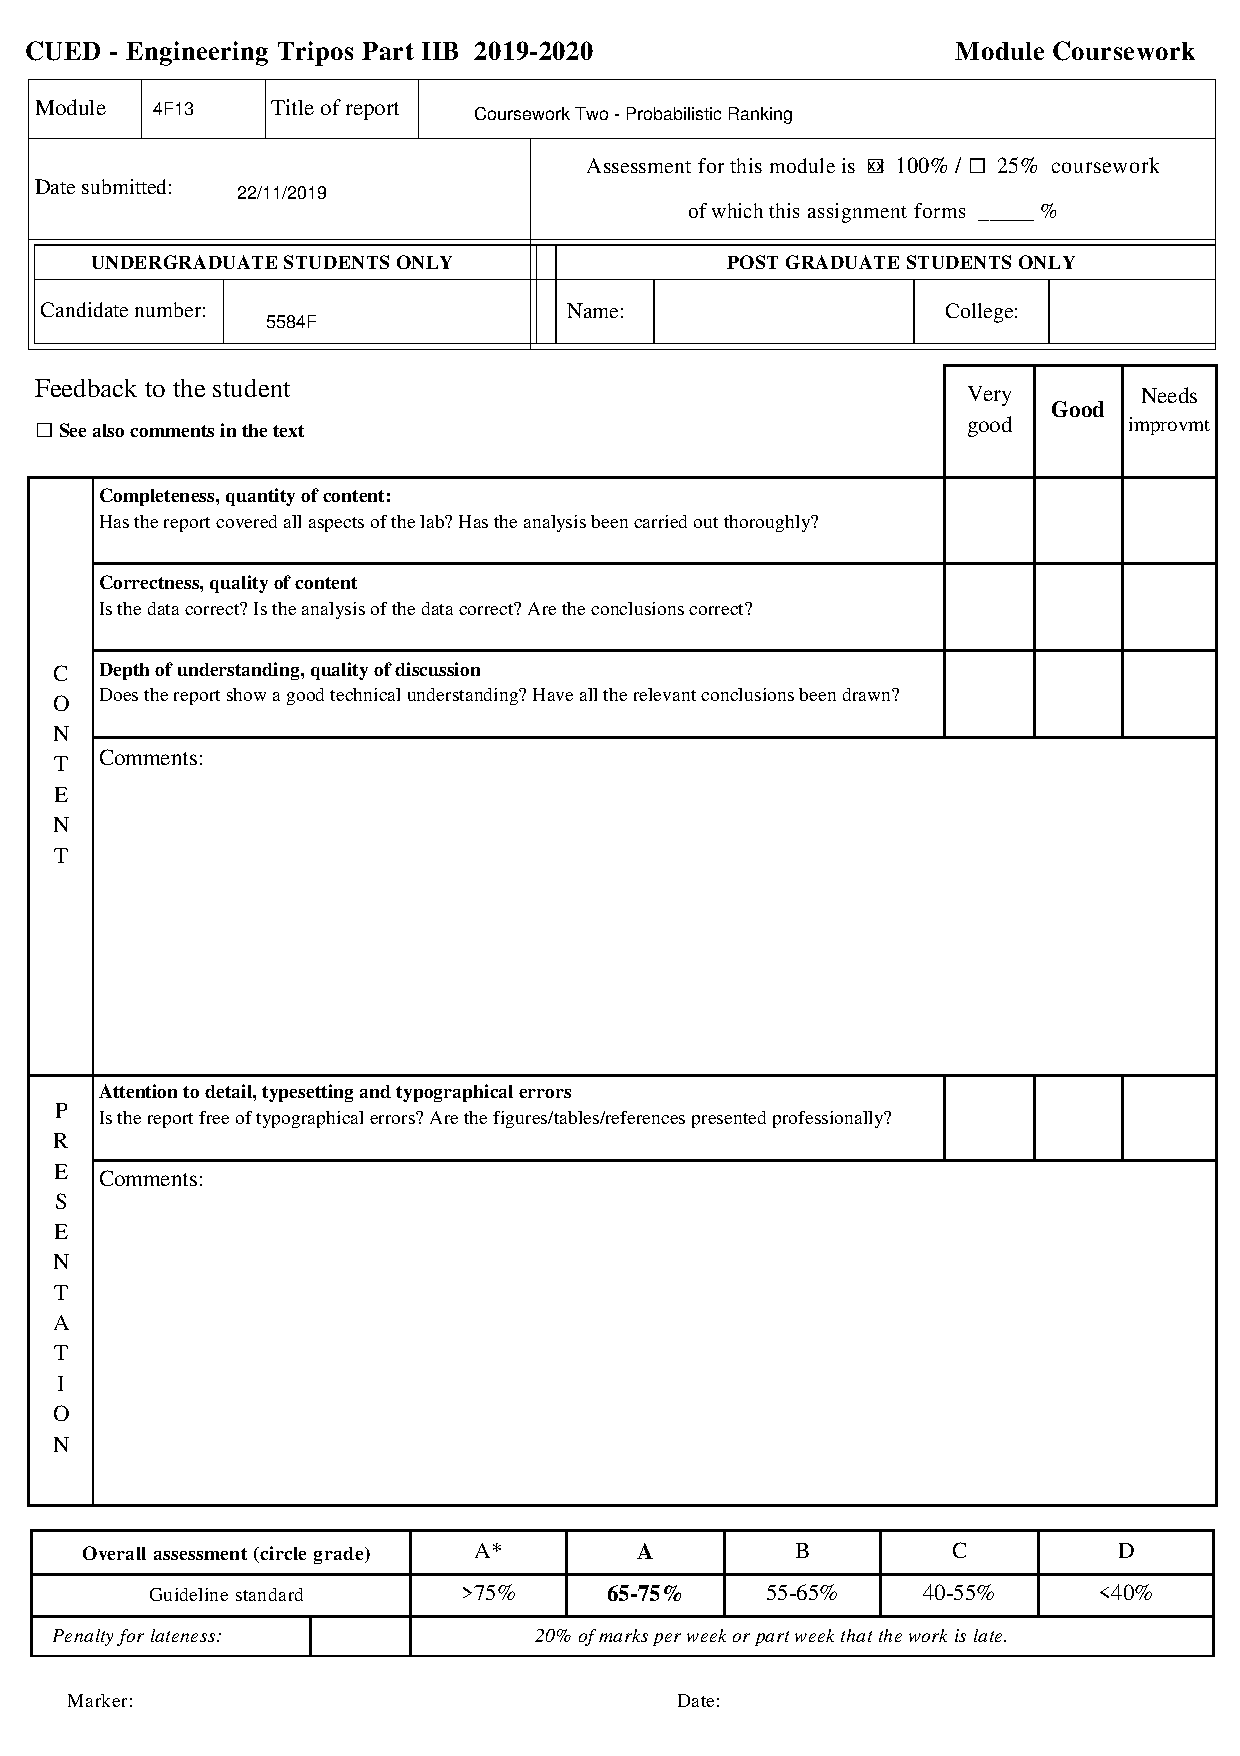
\includepdf[pages={1}]{Coversheet.pdf}
\twocolumn
% Print the title
\maketitle

%----------------------------------------------------------------------------------------
%	ARTICLE CONTENTS
%----------------------------------------------------------------------------------------


\section{a}
\begin{figure}[h]
  \centering
    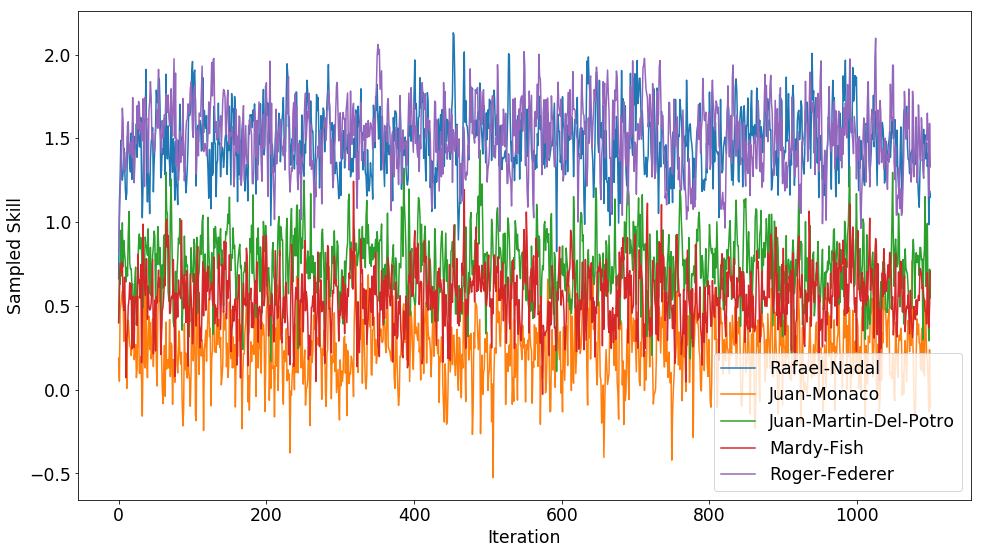
\includegraphics[width=\linewidth]{a_1}
  \caption{Sampled skills from Gibbs sampling}
  \label{fig:a_1}
\end{figure}
Using the data available for tennis matches played and their outcome, the ranking of each players skill and chance of beating another opponent can be calculated. One method of doing this is to use Gibbs sampling. Gibbs sampling is used to jointly sample player skills by sampling from simpler conditional distributions instead of the joint. Figure \ref{fig:a_1} shows these samples being random and different for each player. This method of computing sequential samples leads to dependence between samples. Therefore a burn in time is required after initialising. The burn in is required because the initial variable values may not reside in locating of high probability in the joint distribution, this means several iterations of Gibbs sampling are required for the samples to converge on the desired distribution. Convergence happens when the mean and standard deviation settle which can be found by computing these terms against iteration number. Figure \ref{fig:a_3} shows this convergence, a burn in time of 200 iterations was used in subsequent sampling.
\begin{figure}[h]
  \centering
    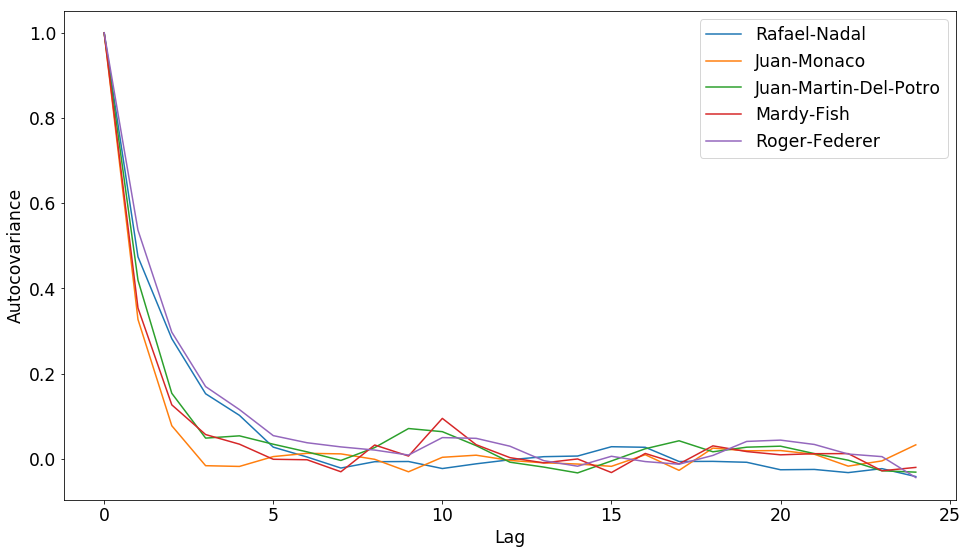
\includegraphics[width=\linewidth]{a_2}
  \caption{Autocovariance of Gibbs sampling}
  \label{fig:a_2}
\end{figure}
Figure \ref{fig:a_2} shows the autocovariance of sampled skills compared to their lag. in order to get independent samples this autocovariance should be 0. A lag of 5 was chosen for sampling independently in later tests. Due to the burn in time and only using 1/5 of all samples the Gibbs sampling algorithm should be run for over 1000 iterations to get enough samples that can be reliably used for ranking.

\begin{figure}[h]
  \centering
    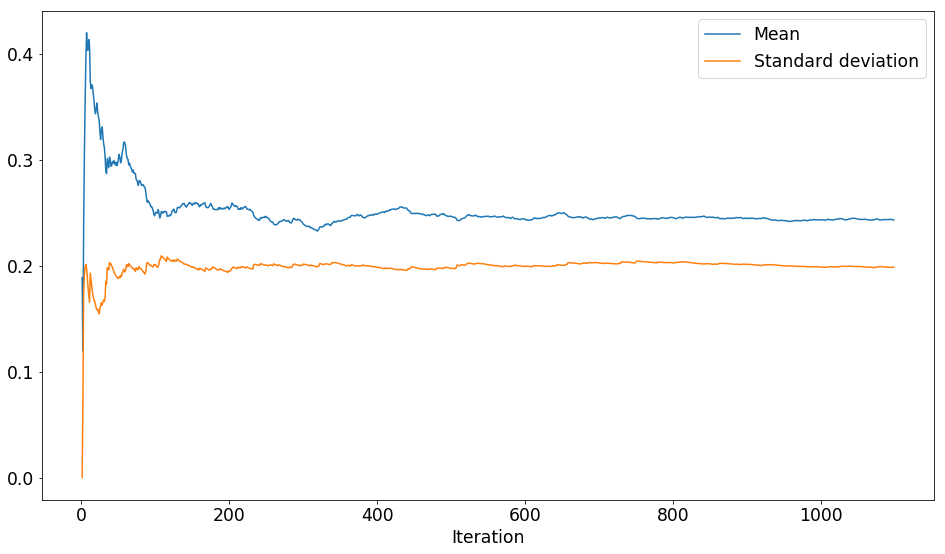
\includegraphics[width=\linewidth]{a_3}
  \caption{Convergence to a distribution}
  \label{fig:a_3}
\end{figure}
%------------------------------------------------
\section{b}
\begin{figure}[h]
  \centering
    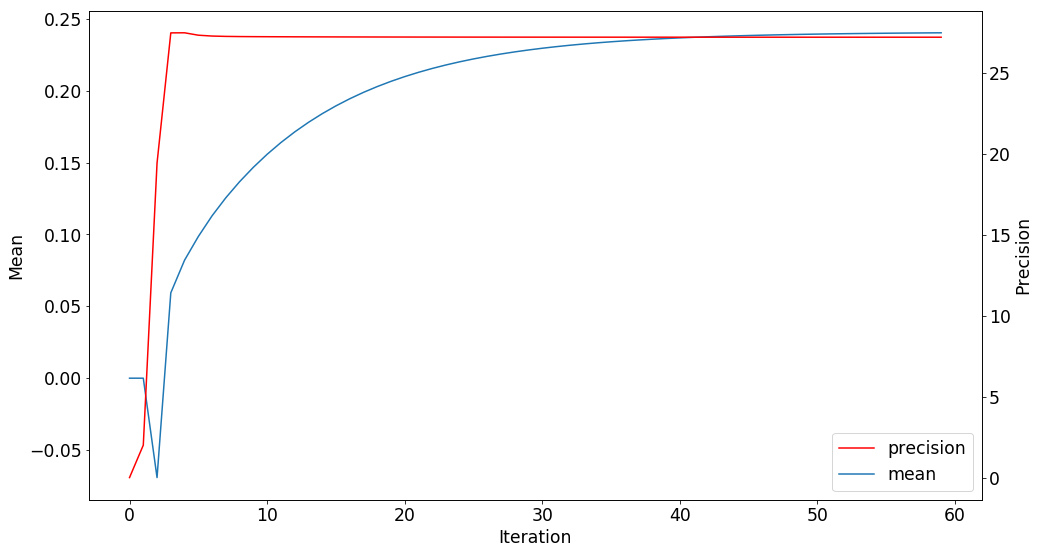
\includegraphics[width=\linewidth]{b_1}
  \caption{Convergence of distribution using message passing}
  \label{fig:b_1}
\end{figure}

Another method of evaluating marginal skill distributions is Expectation Propagation (EP) using message passing. This process involves updating the marginal skill distributions after each instance of propagating the distribution though the factor graphs. Each iteration fits the marginal distributions better to the available game data. 
\newline
The marginal distributions are initialised with a mean and variance, as the message passing iterates these will converge to the desired distribution of skills. Figure \ref{fig:b_1} shows this convergence for one player, the precision settles very quickly within 5 iterations unlike the mean which takes 40 iterations. The number of iterations required will be different for each player as the difference between desired distribution and initial distribution varies. This convergence to a distribution is the same as in Gibbs sampling where the samples converge upon a certain mean and variance.
%------------------------------------------------
\section{c}
\begin{table}[h]
\centering
\begin{tabular}{ c | c  c  c  c}
&ND&RN&RF&AM\\ 

\midrule
ND&0.5  &    0.060 & 0.091 &0.0147\\
RN&0.940&0.5&0.573&0.233\\
RF&0.909&0.427&0.5&0.189 \\
AM&0.985&0.767&0.811&0.5\\
\end{tabular}
\caption{Probability column player has higher skill than row player, using distribution from EP}
\label{table:c1}
\end{table}


\begin{table}[h]
\centering
\begin{tabular}{ c | c  c  c  c}
&ND&RN&RF&AM\\ 

\midrule
ND&0.5  &   0.345 & 0.362 &0.280\\
RN&0.655&0.5&0.518&0.427\\
RF&0.638&0.482&0.5&0.409 \\
AM&0.720&0.573&0.591&0.5\\
\end{tabular}
\caption{Probability column player has higher performance than row player, using distribution from EP}
\label{table:c2}
\end{table}

The top four players on the ATP ranking are Novak Djokovic, Rafael Nadal, Roger Federer and Andy Murray the probability of a players skill and performance being higher then another can be computed using the distributions from EP. The is done by calculating the probability p($skill_1-skill_2$>0), and treating $skill_1-skill_2$ as the random variable. Tables \ref{table:c1} and \ref{table:c2} list these probabilities for skill and game performance respectively. The performance corresponds to the chance a player wins a given game, this is due to the skill difference plus noise. Figure \ref{fig:c_1} shows these distributions between two players. The performance distribution is much wider due to the added uncertainty which results in the less skilled player increasing their chance to win. This is also seen when comparing the probabilities in tables \ref{table:c1} and \ref{table:c2}.

\begin{figure}[h]
  \centering
    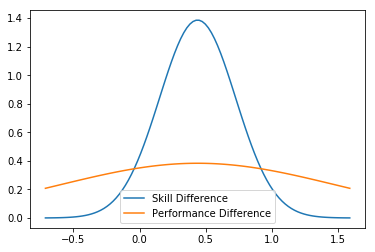
\includegraphics[width=\linewidth]{c_1}
  \caption{Difference between skill and performance for Nadal and Djokovic}
  \label{fig:c_1}
\end{figure}

%------------------------------------------------
\section{d}
\begin{figure}[h]
  \centering
    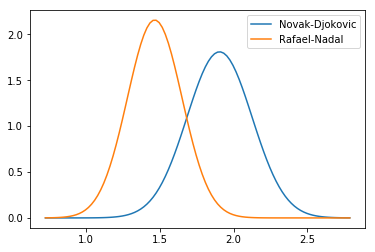
\includegraphics[width=\linewidth]{d_1}
  \caption{Marginal skill distributions with means [1.905, 1.466]$^T$ and standard deviations [0.220, 0.185 ]$^T$ }
  \label{fig:d_1}
\end{figure}

\begin{table}[h]
\centering
\begin{tabular}{ c | c }
Method&p($Djokovic_{s}>Nadal_s$)\\ 

\midrule
Marginal distributions&0.936\\
Joint distribution&0.959\\
From samples&0.972\\
\end{tabular}
\caption{Probability Djokovic has high skill than Nadal computed using three methods }
\label{table:d1}
\end{table}

The skills of two players can be compared using various methods when using Gibbs sampling. The first method is to use the skill marginals, which can be formed by taking the mean and variance of the skill samples and approximating each distribution as normal. The two marginal Gaussians shown in figure \ref{fig:d_1} can then be used to determine the probabilities as before. The Gibbs samples also contain information about the covariance between players, once calculated along with the mean a join distribution can be formed. This is once again approximated to be Gaussian, with the probabilities now calculated from the volume either side of the line $skill_1=skill_2$ as in figures \ref{fig:d_2} and \ref{fig:d_3}. The final method utilises the samples directly, by comparing the skills at a given iteration of the algorithm while ensuring burn in and autocorrelation  times are accounted for. Table \ref{table:d1} shows the probability that Djokovic is more skilled then Nadal for each method, all resulting in similar probabilities.


\begin{figure}[h]
  \centering
    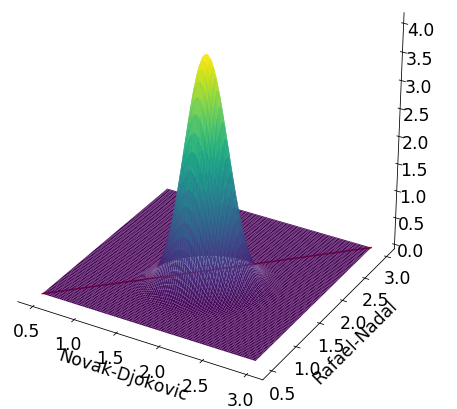
\includegraphics[width=\linewidth]{d_2}
  \caption{Joint skill distribution with means [1.905, 1.466]$^T$, variances [0.0486, 0.0343]$^T$ and symmetric covariance 0.0096}
  \label{fig:d_2}
\end{figure}

\section{d}
\begin{figure}[h]
  \centering
    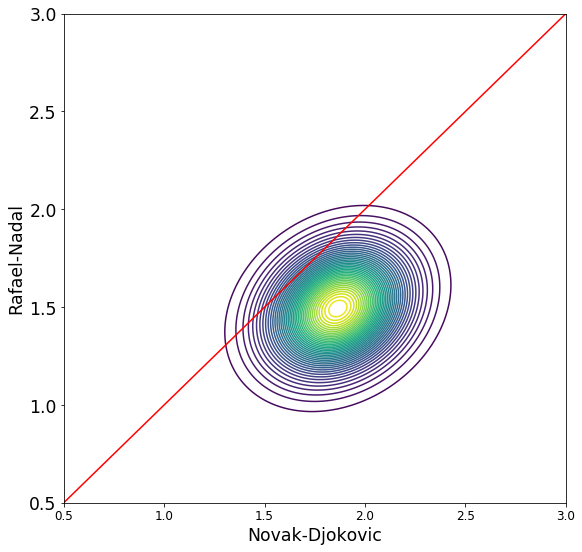
\includegraphics[width=\linewidth]{d_3}
  \caption{Joint skill distribution contour plot }
  \label{fig:d_3}
\end{figure}

Each method has various strengths and downfalls. The marginal distribution and using the samples directly is computationally faster then using a 2D joint Gaussian. However, just using marginal distributions ignores the extra information in the covariance that the other methods take into account, this information contains player pairing specific information. Using the samples directly can result in very noisy probabilities unless lots of samples are used. This means that if the distribution can be reasonably assumed to be Gaussian its best to use the joint distribution as this considers covariance and smooths sample noise. 

\begin{table}[h]
\centering
\begin{tabular}{ c | c  c  c  c}
&ND&RN&RF&AM\\ 

\midrule
ND&0.5  &   0.040 & 0.072 &0.006\\
RN&0.960&0.5&0.579&0.204\\
RF&0.928&0.421&0.5&0.168 \\
AM&0.994&0.796&0.832&0.5\\
\end{tabular}
\caption{Probability column player has higher skill than row player, using joint distribution}
\label{table:d2}
\end{table}
 Table \ref{table:d2} contains the probabilities one player is more skilled then another using the joint Gaussian distribution. Comparing this to table \ref{table:c1} from messaging passing its clear that both methods produce very similar results as all probabilities differ by 0.03 at most. This means the distributions generated with each method are also similar.

%------------------------------------------------------
\section{e}
The ranking of each player can be created using the mean skills of each player from both the message passing and Gibbs sampling. These can be seen in figures \ref{fig:e_2} and \ref{fig:e_3} respectively. These both produce the same ranking, further showing that the converged distributions in each method are similar. Another method of creating a ranking is to calculate the win percentage for each player using the game data. This doesn't take into account how skilled each opponent was in each game, meaning losing to bad players counts as much as losing to good players. Figure \ref{fig:e_1} shows this list. This list depicts a similar overall position for each player, but with lots of the order shuffled slightly meaning player position can differ by around 8 places compared to the other methods. This method is clearly inferior to Gibbs and EP however it is computational faster for generating an approximate list.



\section{Appendix - Code listings}
\subsection{a}
\begin{lstlisting}[language=python]
m[p] = sum(t[np.where(G[:, 0] == p)]) - sum(t[np.where(G[:, 1] == p)]) 
        for g in range(N):
            iS[G[g, 0], G[g, 0]] += 1
            iS[G[g, 1], G[g, 1]] += 1
            iS[G[g, 0], G[g, 1]] -= 1
            iS[G[g, 1], G[g, 0]] -= 1
\end{lstlisting}

\subsection{c}
\begin{lstlisting}[language=python]
def prob_skill_higher(p1,p2,means,pres,performance=0):
    #probability that s1>s2 = p(s1-s2>0) let z=s1-s2 , z~(m1-m2,v1+v2)
    p1=int(p1)
    p2=int(p2)
    mean = means[p1,-1]-means[p2,-1]
    var = 1/pres[p1,-1] + 1/pres[p2,-1] + performance
    prob = 1 - norm.cdf((0-mean)/(var**0.5))
    return prob
\end{lstlisting}
\subsection{d}
\begin{lstlisting}[language=python]
for i in range(2):
    data[i,:] = skill_samples[int(ids[i]),:][burn_in:-1]
    means[i]=np.mean(data[i,:])
 

cov = np.cov(data)
\end{lstlisting}
\onecolumn
\begin{lstlisting}[language=python]
autocov =5
count=0
burn_in=200
it= int((skill_samples.shape[1]-burn_in-1)//autocov )


for i in range(it):
    x1 = skill_samples[int(ids[0]),burn_in + autocov*i ]
    x2 = skill_samples[int(ids[1]),burn_in + autocov*i ]
    if x1>x2:
        count+=1
prob = count/it
\end{lstlisting}

\begin{figure}[h]
  \centering
    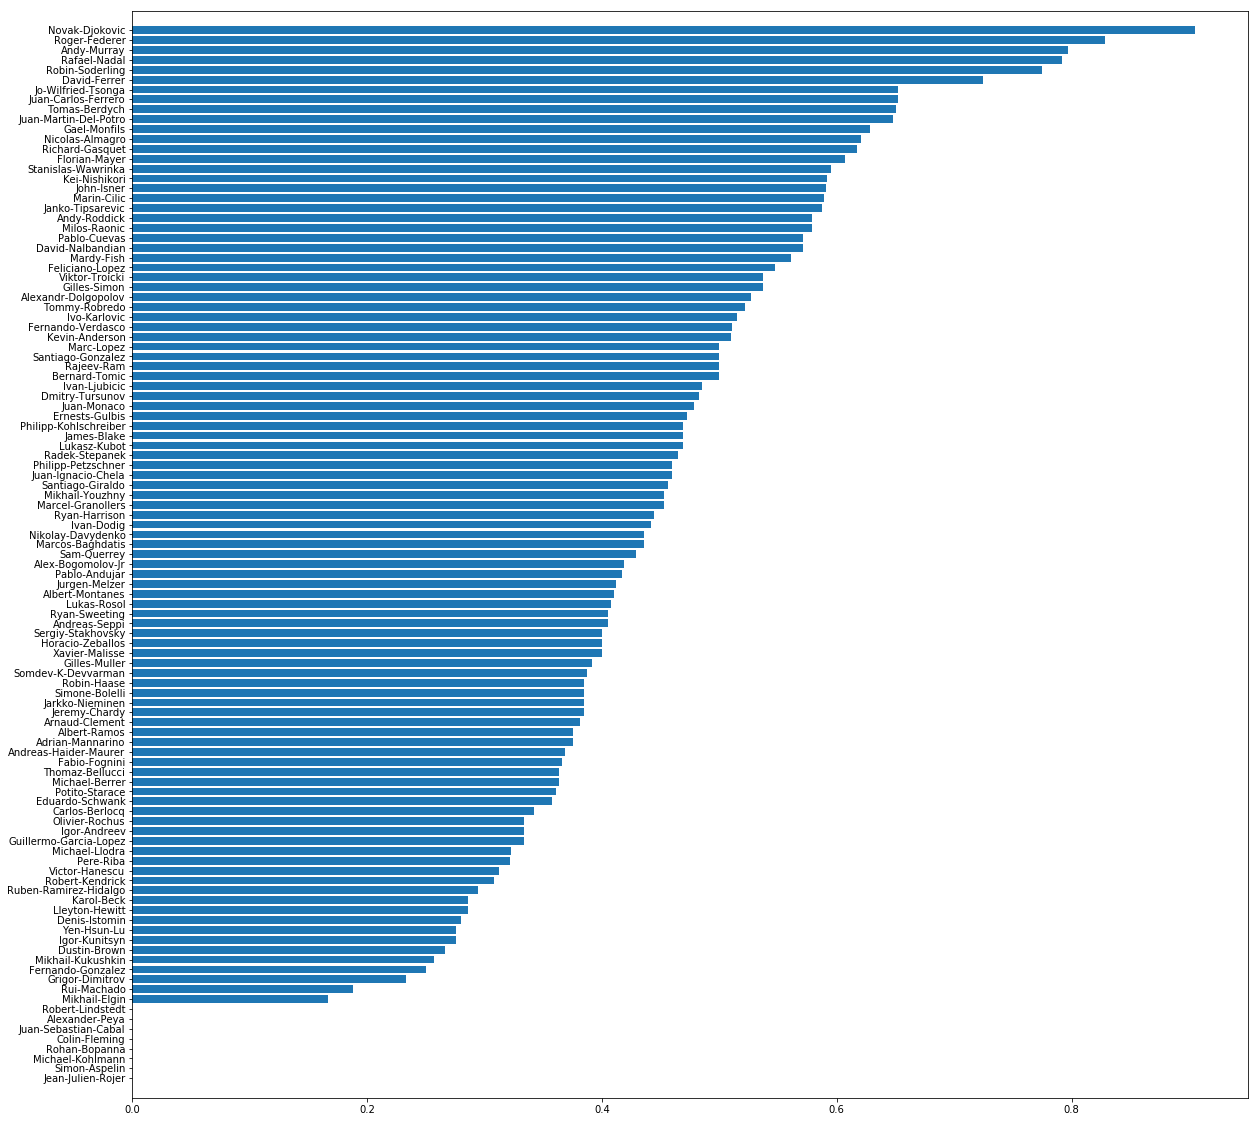
\includegraphics[width=\linewidth]{e_1}
  \caption{Player order using empirical results }
  \label{fig:e_1}
\end{figure}

\begin{figure}[h]
  \centering
    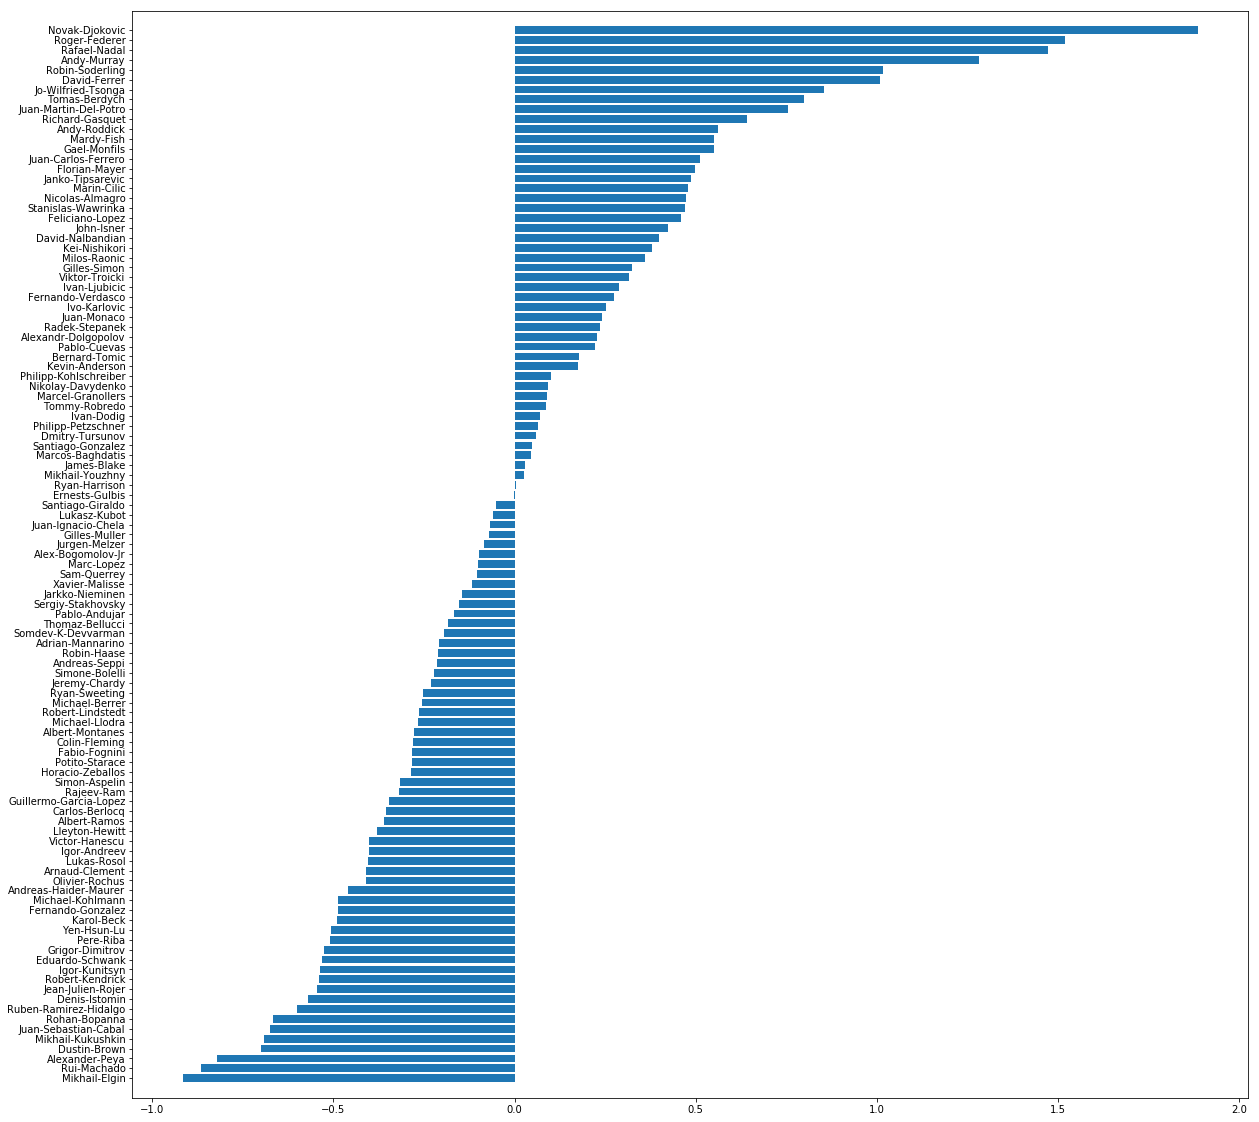
\includegraphics[width=\linewidth]{e_3}
  \caption{Player order using Gibbs sampling }
  \label{fig:e_2}
\end{figure}

\begin{figure}[h]
  \centering
    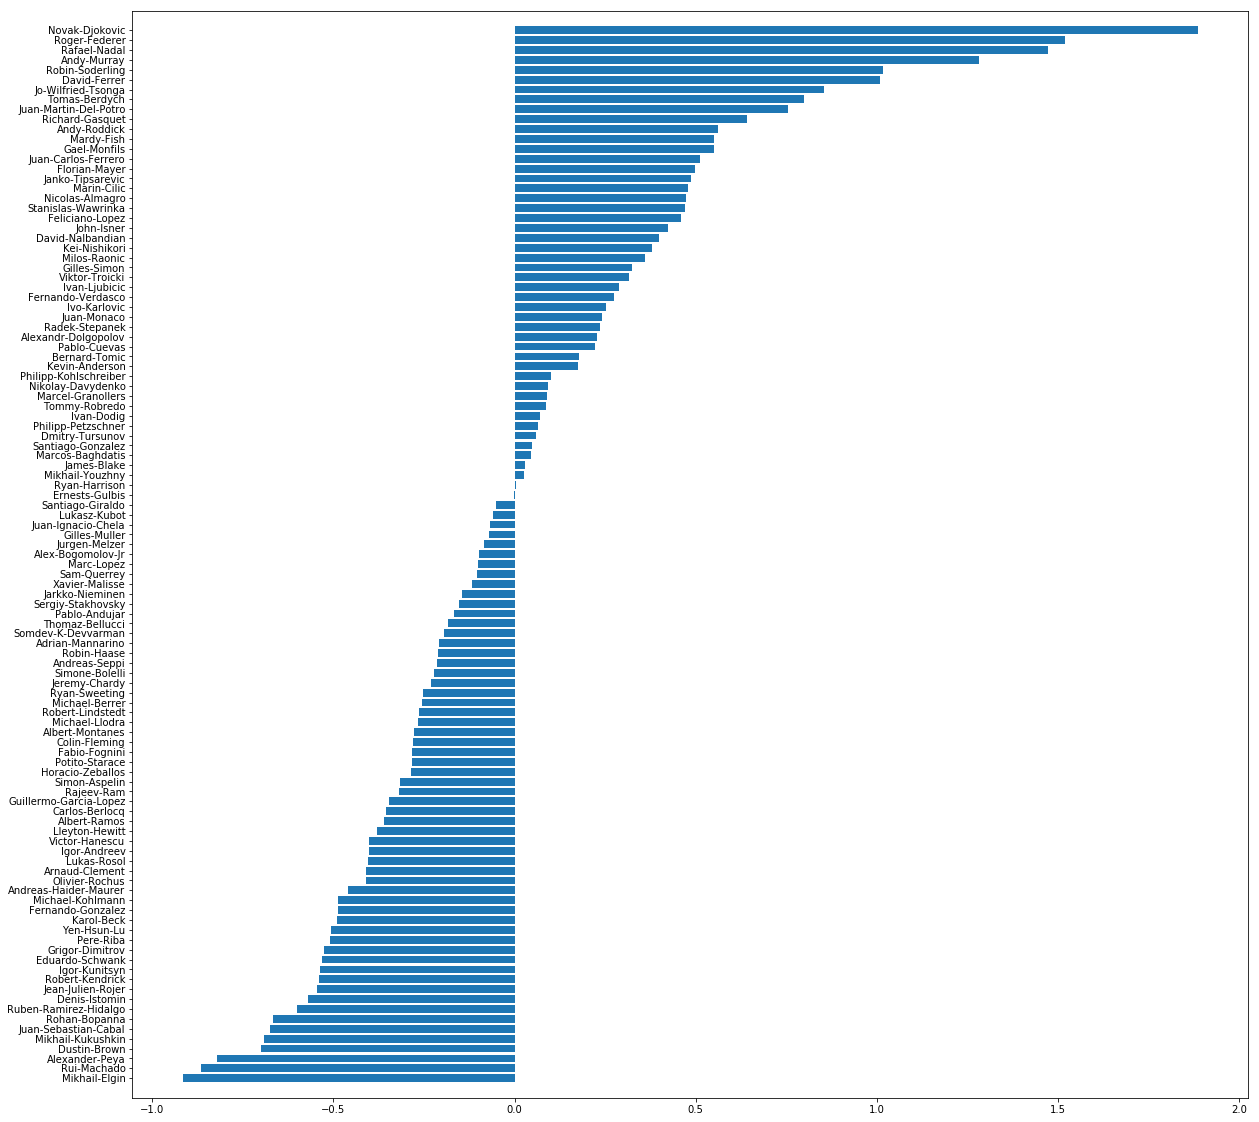
\includegraphics[width=\linewidth]{e_3}
  \caption{Player order using message passing}
  \label{fig:e_3}
\end{figure}
%------------------------------------------------
\end{document}
